% !TeX root = ../main.tex
% Add the above to each chapter to make compiling the PDF easier in some editors.

\section{Design}
\subsection{User Interface Design Styles}
\subsubsection{Material UI}
% MUI Zitate 
% sx Style Properties
The Benchy Viewer's design is rooted in the principles of Material Design, emphasizing a sleek and consistent user interface that aligns with modern design standards.\\
To ensure a cohesive and user-centric design, the application makes extensive use of predefined components from the Material UI framework. This includes buttons, inputs, toggles, sliders, data grids, icons, drop-down menus, and tooltips.

The inclusion of Material Design components contributes to an interface that is both user-friendly and familiar. Users can easily navigate through buttons, toggles, and sliders, thanks to the standardized styling that Material UI provides.

Icons within the Benchy Viewer serve as visual cues, representing familiar symbols that aid users in quickly grasping the functions they perform. This visual clarity aligns with Material Design's emphasis on intuitive iconography.

Settings options, presented in dropdown menus and other interfaces, follow Material Design practices. The design prioritizes user intuition, allowing individuals to interact with the application seamlessly without relying on extensive textual explanations.

By aligning with Material Design principles, the Benchy Viewer achieves a design that not only meets aesthetic standards, but also prioritizes user understanding and interaction efficiency. The incorporation of familiar components enhances the overall usability and accessibility of the application.


\subsubsection{Styling Characteristics}

The Benchy Viewer embraces a deliberate colour scheme aimed at providing a clean design. This is achieved through a restraint to specific base colors, limiting the palette to black, white, and a gray accent colour, as depicted in Figure~\ref{fig:colors}. By adhering to this minimalist approach, the application exudes a sense of simplicity, ensuring a visually uncluttered interface.



\begin{figure}[h]
  \centering
  \includegraphics[width=0.5\linewidth]{figures/colors.png}
  \caption{Colour palette of the user interface.}
  \label{fig:colors}
\end{figure}

While the overall design adheres to a subdued colour palette, the visual elements within the application utilize a distinct colour scheme, as illustrated in Figure~\ref{fig:colors-dbms}. This strategic approach guarantees that charts, plots, and other visual elements command attention, supporting users to focus on those data visualisations.

\begin{figure}[h]
  \centering
  \includegraphics[width=1\linewidth]{figures/colors-dbms.png}
  \caption{Colour palette used by visualisations.}
  \label{fig:colors-dbms}
\end{figure}

To enhance user experience, the Benchy Viewer incorporates immediate feedback mechanisms. When users hover over interactive elements, such as buttons or inputs, accent colours dynamically adjust, providing a visual cue of the interactive nature of the element. Additionally, the mouse representation undergoes subtle changes, reinforcing the responsiveness of the interface.


% Schriftart, Colors (Palette mit Akzenten)

\subsection{Page Structure and Navigation}
\subsubsection{Sidebar}
\subsubsection{Pages}

\section{Data Structure}
\subsection{Overall Project Structure}
\subsection{Input File and Benchmark Data}


\subsubsection{Import of Performance Data}

The first step, working with the Benchy Viewer is to import a file containing the performance data which should be visualised. The file needs to follow the format introduced in Section \ref{sec:input-file-structure}. Figure~\ref{fig:input-process-flow} summarizes the import of the input file in a process diagram.

\begin{figure}[h]
  \centering
  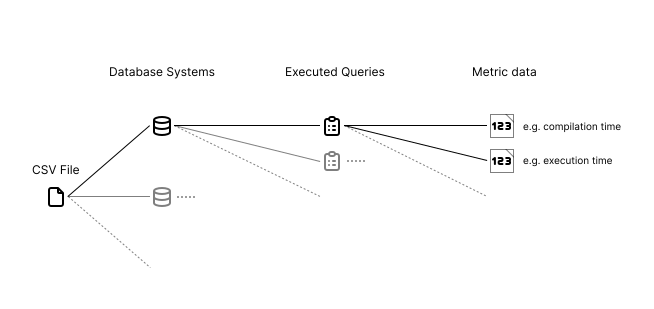
\includegraphics[width=1\linewidth]{figures/csv-structure.pdf}
  \caption{Import process of input data}
  \label{fig:input-process-flow}
\end{figure}

Chart beschreiben.


\subsection{Plot Options}
\subsection{Visualisation Arrangement Data Structure}
\subsection{Query Plan}
\subsubsection{Visualisation Parameters}
\subsubsection{Query Plan Data Structure}

\section{Integration of Plotly-React for Data Visualisation}
\subsection{Types of Plots and Charts}
\subsection{Hover Feature}
\subsection{Selected Query Feature}

\section{Integration of semantic-diff-tool}\label{sec:semantic-diff-integration}
\subsection{Business Logic}
\subsection{Settings}
\subsection{UI}